\subsection{A control with exactly fixed charge geometry}\label{sec:rigid}

To separate intrinsic geometry from angular coupling, we constructed an independent unpaired
particle--rotor control with $j=11/2$, fixed triaxiality
$\gamma=20^\circ$ and a core-only electric tensor
\begin{align}
T_{2\mu}(\Omega)&=\mathcal Q\sum_\nu D^{2*}_{\mu\nu}(\Omega)a_\nu,
\label{eq:rigidcharge}\\
a_0&=\cos\gamma,\qquad a_{\pm2}=\frac{\sin\gamma}{\sqrt2}.\nonumber
\end{align}
The remaining intrinsic components vanish. Because these are
multiplication operators on rotor orientation, the standard tensor
contractions give the pointwise identities
\begin{equation}
T\cdot T=\mathcal Q^2\mathbf1,\qquad
-\sqrt{\frac72}[T\times T]^{(2)}\cdot T
=\mathcal Q^3\cos3\gamma\,\mathbf1.
\label{eq:rigididentity}
\end{equation}
They hold independently of the particle--rotor eigenstate. We set
$\mathcal Q=1$ and quote moments in the corresponding amplitude units.
The complete ratio is therefore exactly $1/2$ and its angle $20^\circ$.

The Hamiltonian retains fixed irrotational inertias while the coefficient
$C$ of a declared quadrupole single-particle field takes the preselected
values 0, 1, 2, 4 and 8 MeV. The field changes angular coupling but neither
the tensor in Eq.~(\ref{eq:rigidcharge}) nor its geometry.
Appendix~\ref{app:rigid} specifies the field normalization, body-axis
convention and physical $D_2$ space. This is an illustrative control,
with no Ba fit and no identification of $C$ with the IBFM's $\Gamma_0$.

Figure~\ref{fig:rigid} shows that the all-$15/2$ selected ratio increases
from 0.32262 to 1.02625 while both complete moments remain fixed.
All 48 physical $15/2$ states are included, so the final domain failure
survives removing the state-count restriction within that spin.
The corresponding static fraction grows from zero to 35.95\%.
Thus a change in angular correlations can alter this converged diagnostic
without changing intrinsic charge shape. This result does not establish
unchanged geometry in the separate IBFM calculation.

\begin{figure*}[t]
\centering
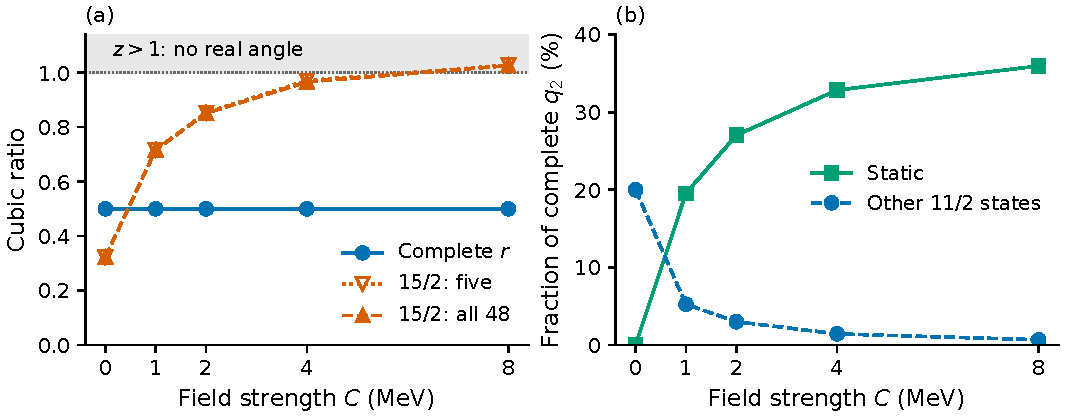
\includegraphics[width=\textwidth]{figures/rigid_charge_control-v1.pdf}
\caption{Independent rigid-charge particle--rotor control at
$\gamma=20^\circ$. (a) Complete ratio and selected-channel ratios using
five or all 48 $15/2$ states. (b) Static and other-same-spin fractions of
$q_2$. The intrinsic tensor and inertias remain fixed at every point;
$C$ has the normalization of Appendix~\ref{app:rigid}.
The shaded region marks the absence of a real selected angle.
Lines join the five calculated points and do not assert untested
continuous-parameter behavior.}\label{fig:rigid}
\end{figure*}

The charge identities were checked as matrices on the entire initial
$11/2$ space, with maximum residual $5.6\times10^{-16}$, and against
independent Euler-angle integration of tensor elements.
All required intermediate spins for its quadratic and cubic closure
are present. Numerical branch matching retains the lowest $11/2$
state in both directions, with minimum adjacent squared overlap 0.648.
The exact geometric identity does not depend on extrapolating that
sampled tracking into a continuous no-crossing claim.
